\documentclass{report}
\usepackage{bbold}
\usepackage{amsmath}
\usepackage[margin=.75in]{geometry}
\usepackage{graphicx}
\usepackage{color}

\sloppy
\definecolor{lightgray}{gray}{0.5}
\setlength{\parindent}{0pt}

\begin{document}
ENEE 324 HW \#4 \\
Jacob Besteman-Street \\
\today \\
\begin{enumerate}
\item Suppose that a random variable (RV) $Y$ has the following cumulative distribution function (CDF): \\
$$ F_Y(y) = \left. \begin{cases}
0 & if y < 1 \\
\frac{1}{8}(y-1)^3 & if 1 \leq y < 3 \\
1 & if y \geq 3
\end{cases} \right.$$
\begin{itemize}
  \item[(a)] Find and sketch the probability density function (PDF) of RV $Y$. \\
  The PDF is the derivative of the CDF.
  $$ PDF = f_Y(y) = \left. \begin{cases}
  0 & if y < 1 \\
  \frac{3}{8}(y-1)^2 & if 1 \leq y < 3 \\
  0 & if y \geq 3
  \end{cases} \right.$$
I could sketch this by hand, but it looks better this way. Using Matlab:
\begin{verbatim}
syms y(x);
y(x) = piecewise(x<1, 0, 1<x<3, (3/8)*(x-1)^2, x>3, 0);
fplot(y, [0,4])
\end{verbatim}
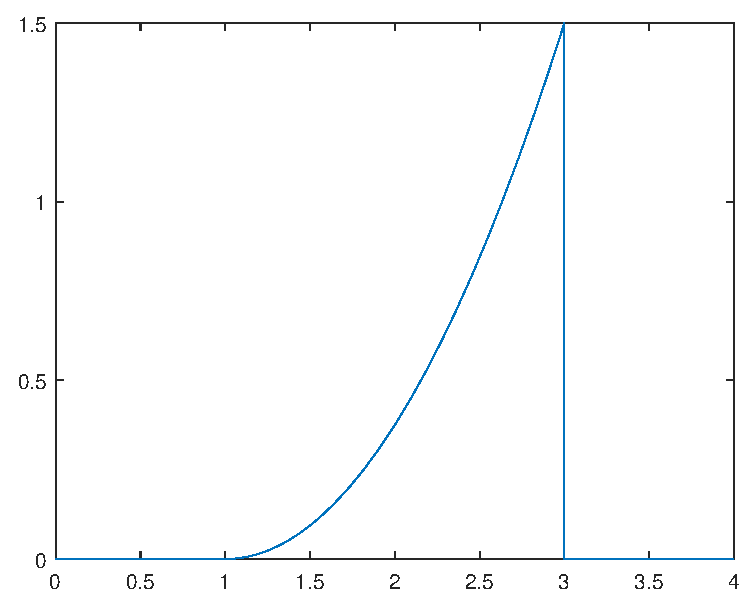
\includegraphics [width=4in]{enee324hw4_01.eps}

  \item[(b)] Compute $P[0.5<Y \leq 2.5 ]$ \\
  $$ P[0.5<Y \leq 2.5 ] = \int_{0.5}^{2.5} f_Y(y) dy = \int_{1}^{2.5} {3}{8}(y-1)^2 dy = \frac{1}{8}(y-1)^3 \text{ at } y=2.5 = 0.421875 $$
  \item[(c)] Compute $E[Y]$ and $Var(Y)$. \\
  $$ E[Y] = \int_{-\infty}^{infty}y \cdot f_Y(y) dy = \int_{1}^{3} \frac{3y}{8}(y-1)^2 dy = \int_{1}^{3} \frac{3}{8}(y^3 - 2y^2 + y) dy = [\frac{3}{32}y^4 - \frac{1}{4}y^3 + \frac{3}{16}y^2]_{1}^{3} $$
$$ = [\frac{243}{32} - \frac{27}{4} + \frac{27}{16}] - [\frac{3}{32} - \frac{1}{4} + \frac{3}{16}] = [\frac{243}{32} - \frac{216}{32} + \frac{54}{32}] - [\frac{3}{32} - \frac{8}{32} + \frac{6}{32}]  = \frac{81}{32} - \frac{1}{32} = \frac{80}{32} = 2.5 = E[Y]   $$
To find $Var(Y)$, need $E[Y^2]$.
$$ E[Y^2] = \int_{-\infty}^{infty}y^2 \cdot f_Y(y) dy = \int_{1}^{3} \frac{3y^2}{8}(y-1)^2 dy = \int_{1}^{3} \frac{3}{8}(y^4 - 2y^3 + y^2) dy = [\frac{3}{40}y^5 - \frac{3}{16}y^4 + \frac{1}{8}y^3]_{1}^{3} $$
$$ = [\frac{729}{40} - \frac{243}{16} + \frac{27}{8}] - [\frac{3}{40} - \frac{3}{16} + \frac{1}{8}] = [\frac{1458}{80} - \frac{1215}{80} + \frac{270}{80}] - [\frac{6}{80} - \frac{15}{80} + \frac{10}{80}] = \frac{513}{80} - \frac{1}{80} = \frac{512}{80} = 6.4 = E[Y^2] $$
$$ Var[Y] = E[Y^2] - E[Y]^2 = 6.4-6.25 = 0.15 $$
\end{itemize}
\item Rachel drives to the BWI airport to see off a friend. She can park her car in one of two hourly
parking garages. The parking garages charge \$1 per hour. However, the first parking garage charges
for full hour for any fraction, even if the car is parked only for 1 second, while the second parking
garage charges only for the amount of time the car is parked there. Rachel will park for $Y$ number of
hours, where $Y$ is exponentially distributed with parameter 0.3. Let $Z$ be the amount Rachel pays for
parking.
\begin{itemize}
    \item[(a)] Suppose that Rachel parks her car at the first parking garage. Compute the PMF of RV $Z$ and $E[Z]$.\\
    $Z$ is geometric, starts at a value of 1, and has a parameter of $p= 0.3$.
    $$ p_Z(z) = \left. \begin{cases}
    (0.7)^{z-1}(0.3) & for z = 1,2,3... \\
    0 & otherwise
    \end{cases} \right.$$
    The expectation for a geometric RV is $\frac{1}{p}$, so $E[Z] = 0.3^{-1} = 3.33$
\item[(b)] Suppose that Rachel goes to the second parking garage instead. What is $E[Z]$?\\
In this case, $Z = \$ 1 \times Y$, so $Z$ is an exponential distribution with parameter $ \lambda = 0.3$ and expectation $E[Z] = \lambda^{-1} = 3.33$. I'm not sure I did this right, because it seems like Z should be higher for the first garage, yet the expecatation is the same.
\end{itemize}
\item Pam takes the shuttle bus back to her place after school. Suppose that the waiting time for the shuttle
bus in minutes is an exponential RV $Z$ with parameter $\lambda = 0.1$.
\begin{itemize}
  \item[(a)] Compute the probability $P[A | B]$, where $A = \{Z > 5 minutes\}$ and $B = \{Z > 2 minutes\}$. \\
  Exponential RVs are memoryless. Therefore, $P[\{Z > 5 minutes\} | \{Z > 2 minutes\}] = P[\{Z > 3 minutes\}] $
  $$P[\{Z > 3 minutes\}] = \lambda e^{-3\lambda } = 0.1e^{-0.3} = 0.0741$$
  \item[(b)] Suppose that Pam has waited for the shuttle bus for 5 minutes, but the shuttle bus did not show
up. Given this, what is the conditional expected value of $Z$? \\
Again, exponential functions are memoryless, therefore the time waiting has no impact on how soon the bus will come. The normal expected value of $Z$ is $E[Z] = 0.1^{-1} = 10$. If it hasn't come for 5 minutes, that is added on and the
new expected value is 15 minutes.
\end{itemize}
\item Consider an optical fiber transmission line that uses unipolar nonreturn-to-zero signaling (also called
on-off signaling). When bit 1 is sent, the signal we send is $m > 0$ and when bit is 0, we send
0. When a maximum likelihood detector is used, the probability of bit error (called bit error rate) is $Q\frac{\alpha \cdot m}{ 2\sigma}$,
 where $\alpha$ is the signal attenuation and $\sigma^2$ is the noise variance. Suppose that $\alpha = 10^{−4}$. [For
this problem you will need the table of Φ or $Q$ function posted along with the homework assignment.]
\begin{itemize}
  \item[(a)] Assume $\sigma^2 = 10^{-6}$. What is the minimum required value of $m$ if we want to ensure that the bit error rate does not exceed $10^{-4}$?
  \item[(b)] If $m=1$, hat is the maximum noise  variance we can tolerate subject to the same constraint that the bit error rate does not exceed $10^{−4}$?

\end{itemize}
\item  In the Internet, messages (e.g., emails) are broken into smaller pieces, called packets, before being
transmitted. Packets are lost at a router (switch) due to limited buffer (physical memory) at the router.
Let $T_i, i = 1, 2, \cdots,$ denote the time at which i-th packet loss occurs with $T_0 = 0$ and $X_i = T_i − T_{i−1}$
be the inter-loss time between the \textit{i}-th and (\textit{i}−1)-th packet losses (as shown in Figure 1). Suppose that
the inter-loss times $X_i, i = 1, 2, \cdots ,$ are independent and exponentially distributed with parameter $λ$,
i.e., $X_i$ ∼ exponential(λ) for all $i = 1, 2, \cdots$.
\begin{itemize}
\item[(a)] Let $N$ be the number of packet losses that occur during the interval [0, 2]. Find the PMF of RV
$N$ and compute $E[N]$.
\item[(b)] Compute the probability $P[T_4 \leq 4]$.
\end{itemize}
\item  Suppose a RV $X ∼ N(\mu, \sigma^2)$. We define Y = $g(X) = e^X$. Compute the PDF function of the RV $Y$ .

\end{enumerate}
 \end{document}
